\documentclass{beamer}

\usepackage{fontspec} 
\usepackage{lsp-makros}
\useoutertheme{lsp}

\usepackage{lsptitle}
\usepackage{mdframed}
\def\two@digits#1{\ifnum#1<10 0\fi\number#1}
\def\mytoday{\two@digits{\number\day}.\two@digits{\number\month}.\number\year}


\usepackage{xspace,multicol}
\newcommand{\latex}{\LaTeX\xspace}
\usepackage{tikz}


\newcounter{lastpagemainpart}
\footnotesep0pt
\renewcommand{\footnoterule}{}
\usefootnotetemplate{
  \noindent
  \insertfootnotemark\insertfootnotetext}

\let\beamerfn=\footnote
\renewcommand{\footnote}[1]{%
\let\oldfnsize=\footnotesize%
\let\footnotesize=\tiny%
\beamerfn<\thebeamerpauses->{#1}%
\let\footnotesize=\oldfnsize}


\date{\today}

\usepackage{eurosym}  
 
\renewcommand{\centerline}[1]{\hfill#1\hfill\hfill\mbox{}}


\title{\mbox{Auf der Suche nach dem 'Kunden'} \large Globaler Nutzen \& lokale Kosten}

% \institute{FU Berlin}
\author[LangSci]{Sebastian Nordhoff \& Debora Siller}


\newlength{\distlength}
\setlength{\distlength}{.7mm}

\newcommand{\saeule}[1]{
\fbox{\parbox[b][#1\distlength][b]{1cm}{\centering #1\\[1mm]}}
}

\newcommand{\distribution}[4]{
\parbox[b][\textheight][b]{\textwidth}{
  \centering 
\setlength{\fboxsep}{0pt}
\saeule{#1}
\saeule{#2}
\saeule{#3}
\saeule{#4}
}
}
 



\begin{document}
\lspbeamertitle
\frame{ 
\frametitle{Outline}
\tableofcontents
}

\section{Einleitung}
\frame{ 
\frametitle{Einleitung} 
\begin{itemize}
 \item Language Science Press
 \item Sprachwissenschaft

	Bücher zwischen 100 und 800 Seiten. 
	Tieferes technisches Verständnis kann nicht vorausgesetzt werden

 \item Bücher. 9 publiziert, 111 Anfragen
 \item langsci-press.org
 \item Bedingung: Entwicklung eines Geschäftsmodells
\end{itemize} 
}
 
\section{Kosten}
\frame{ 
\frametitle{Geschäftsmodell} 
\begin{itemize}
 \item Vision
 \item Kosten 
 \item Akteure 
 \item Einnahmearten 
 \item Berechnungen
\end{itemize} 
}

 
\frame{ 
\frametitle{Kosten}
\begin{columns}
\column{5cm}
\begin{itemize}
 \item Personal 
 \item Sachkosten
\end{itemize}
   \begin{itemize}
 \item    Derzeit ca. 10k€/Buch
\item perspektivisch 3.5k€
\item {\LaTeX}-Satz autorenseitig
\end{itemize}
\column{5cm}
\saeule{60}
\saeule{40}
\end{columns}
}

\frame{ 
\frametitle{Kostenberechnung}
\begin{itemize}
 \item ca. 40 Variablen 
 \item \textbf{bekannt}: Tariftabellen, Steuersätze, Supporter
 \item \textbf{gut schätzbar}: Aufwand einzelner Arbeitschritte, Einreichungszahlen 
 \item \textbf{unbekannt}: Spendenbereitschaft, Fördermitgliedschaften, Autorengebührenquote
\end{itemize}
} 
 

\frame{ 
\frametitle{Kostenverteilung} 
\begin{itemize}
 \item Autorenbetreuung 40\% 
 \item Hrsg-Betreuung 8\%
 \item long tail: Feinsatz, Koordinierung PoD, Ausstattung, IT, Design, Marketing, Reise, Rechtsberatung, Steuerberatung, Verbrauchsmaterialien, Dokumentation,  strategische Planung, Mittelakquise, \dots	
\end{itemize}
 
\saeule{40}
\saeule{8}
\saeule{6}
\saeule{5}
\saeule{5} 
\saeule{4} 	
}
 
    
\frame{ 
\frametitle{Vergleich zu Kosten anderer Verlage}
\begin{itemize}
 \item geringe Kosten
\begin{itemize}
 \item Rechtsberatung: keine komplizierten Autorenverträge durch CC-BY 
 \item IT: keine aufwendige Zugangskontrolle, kein DRM, keine Rechnungslegung
 \item http://bjoern.brembs.net/2014/07/are-we-paying-us3000-per-article-just-for-paywalls/
\end{itemize} 
 \item kalkulatorische Schätzwerte können eingesehen werden   
\end{itemize}

}

     

\section{Gruppen}
\frame{ 
\frametitle{Gruppen} 
\begin{itemize}
 \item  Autoren
 \item  Leser
 \item  Bibliotheken 
 \item  Universitäten 
 \item  Fachgesellschaften 
 \item  (Staat) 
\end{itemize} 
} 
 

\section{Wertversprechen}
\frame{ 
\frametitle{Wertversprechen}
\begin{itemize}
 \item  Autoren $\to$
 \item  Leser $\to$
 \item  Bibliotheken  $\to$
 \item  Universitäten  $\to$
 \item  Fachgesellschaften  $\to$
 \item  (Staat)  $\to$
\end{itemize} 
}
 
\section{Einnahmearten}

\frame{ 
\frametitle{} 
\begin{itemize}
 \item  Publikationsgebühren 
 \item  Individualmitgliedschaften 
 \item  institutionelle Mitgliedschaften 
 \item  Spenden 
 \item  Printmarge 
 \item  (Grundfinanzierung)
\end{itemize} 
Je mehr Einnahmearten, desto mehr Verwaltungsaufwand!
}

 


\section{Rechtliches}

      \frame{ 
\frametitle{Juristisches Horrorkabinett}
\begin{itemize}
 \item  sind Gebühren steuerpflichtig?
 \item  können wir Spendenbescheinigungen nach norwegischem Recht ausstellen?
 \item  sind anonyme Spenden via Flattr o.ä. mit deuschen Verwaltungsvorschriften vereinbar?
 \item  wie können Printmargen verbucht werden, wenn diese vom Dienstleister in den USA in USD angewiesen werden, bei der Uni aber in EUR ankommen und der Dienstleister sich weigert, die Kostenstelle in den Betreff der Überweisung zu schreiben?
\end{itemize}
$\Rightarrow$     ab welcher Höhe deckt eine Spende ihren Verwaltungsaufwand?
   \begin{itemize}
 \item    Reduzierung des Verwaltungsaufwandes durch Gründen eines Fördervereins
\end{itemize}

}
 
\frame{ 
\frametitle{Rechtsform}
\begin{itemize}
 \item Die Unternehmung sollte agil handeln können
 \item Die Unternehmung soll betriebswirtschaftlich verantwortlich handeln 
 \item Die Unternehmung soll kostendeckend arbeiten
 \item Die Rechtsform sollte AUF KEINEN FALL profitorientiert sein
  \begin{itemize}
    \item Verkauf von Prestige 
  \end{itemize}
\end{itemize}
}

\section{Kostenverteilung}

\frame{ 
\frametitle{Verteilung} 
\distribution{25}{25}{25}{25}
}

\frame{ 
\frametitle{Verteilung}  
\distribution{10}{30}{20}{40} 
}

\frame{ 
\frametitle{Verteilung}   
\distribution{50}{0}{0}{50} 
}
\frame{ 
\frametitle{Verteilung}   
\distribution{80}{0}{10}{10} 
}


\frame{ 
\frametitle{Verteilung}   
\distribution{43}{18}{16}{23} 
}

\frame{ 
\frametitle{Verteilung}   
\distribution{0}{0}{0}{0} 
}

\section*{Danke}

\frame{ 
\frametitle{Evaluation} 
\begin{itemize}
 \item Die derzeitigen Annahmen sind ungenau
 \item Nachjustierung, sobald genauere Zahlen verfügbar werden
 \item Eventuell Anpassung der Strategie
\end{itemize} 
} 

\frame{ 
\frametitle{Vielen Dank}
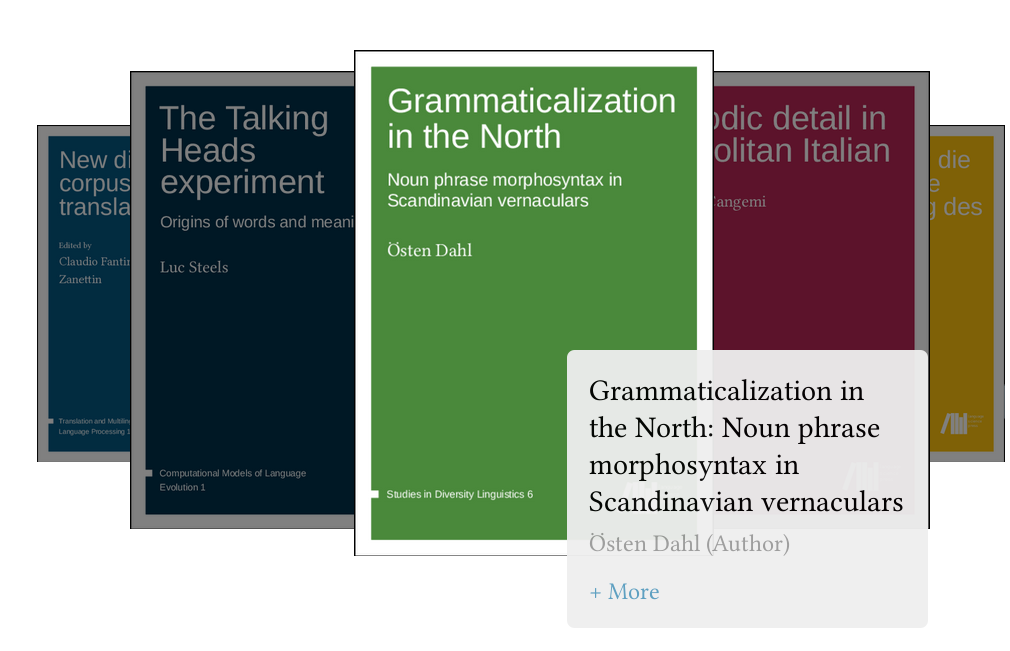
\includegraphics[height=1\textheight]{pics/catalog.png}
}

% OLH
% Edition Open Access
 
\end{document}
